\documentclass[letterpaper,12pt]{extarticle}%Preambulo
\usepackage[utf8]{inputenc}%Preambulo
\usepackage[spanish,mexico]{babel}%Preambulo
\usepackage{ae}
\usepackage{amsmath,amssymb,amsfonts,latexsym,cancel}%Preambulo
\usepackage{hyperref}%Preambulo
\usepackage[pdftex]{graphicx}%Preambulo
\usepackage{wrapfig}%Preambulo
\usepackage[rflt]{floatflt}%Preambulo
\usepackage{fancyhdr}%%Pre?mbulo
\usepackage{mathptmx}%%Pre?mbulo
\usepackage{float}%%Pre?mbulo
\usepackage{longtable,multirow,booktabs}%%Pre?mbulo
%\usepackage{cite}
\usepackage{wrapfig}%%Pre?mbulo
\usepackage[rflt]{floatflt}%%Pre?mbulo
\usepackage{natbib} %%Pre?mbulo
\usepackage{multicol}%%Pre?mbulo
\usepackage{caption}%%Pre?mbulo
\usepackage{geometry}
\usepackage{wrapfig}
\usepackage{adjustbox}
\usepackage{amsmath}
\usepackage{parskip}
\usepackage{tikz}
\usepackage{lipsum}
\usepackage{xcolor}
\usepackage[T1]{fontenc}

\captionsetup{
       font=small,
       labelfont=bf,
       tableposition=top,
       hypcap=false
    }

\DeclareGraphicsExtensions{.pdf, .png, .jpg, .PNG, .JPG}%Cuando ponemos im?genes ya no es necesario poner la extensi?n

%%%FORMATO DE LA P?GINA%%%
\textheight = 21cm %Medidas de la  p?gina
\textwidth = 18cm  %Medidas de la p?gina
\topmargin = -1cm  %Medidas de la p?gina    
\oddsidemargin = -1cm %Medidas de la p?gina
\pagestyle{fancy} %Dise?o de la p?gina
\lhead{Universidad de la Sierra Sur}%%LeftHead
\chead{
\includegraphics[width=1cm, height=1cm]{imag//logL}}%%CenterHead
%\lfoot{USM}
\rhead{Licenciatura en Informática}%%RightHead
%\lfoot{Gonz?lez Chico Juan Daniel} %Pie de pagina izquierdo

\setlength{\columnsep}{7mm}%Comandos para el formato de la p?gina
%\setlength{\parindent}{4em}%Sangr?a al comenzar un nuevo p?rrafo
\setlength{\parindent}{0.5in}
%\setlength{\parindent}{4em}%Sangr?a al comenzar un nuevo p?rrafo
\setlength{\parskip}{1em}%distancia entre p?rrafos
\renewcommand{\baselinestretch}{1.0}% Espacio entre l?nea y l?nea
\setlength{\headheight}{33pt}

\hypersetup{
	colorlinks = true,
	linkcolor = black,
	urlcolor = cyan
}
\urlstyle{same}

\begin{document}

    \begin{titlepage}
		% Mine page for add image at scale with footer image in 
		\begin{figure}[ht]
		   \minipage{0.76\textwidth}
				
\includegraphics[width=4cm]{imag//logColor.jpg}
				\label{escudoFI}
		   \endminipage
		   \minipage{0.32\textwidth}

				
\includegraphics[height = 4.5cm ,width=4cm]{imag//logBN.jpg} 
				\label{EscuoUNAM}
			\endminipage
				%%\vspace{-1cm}
		\end{figure}
		
		\vspace{0.5cm}
		
		\begin{center}
			\LARGE UNIVERSIDAD DE LA SIERRA SUR \\
			\vspace{0.3cm}
			\LARGE Instituto de Informática
			
			\vspace{.7cm} {\LARGE  \textbf{Programa de conversión de bases} \\}

			% Incrementamos el interlineado:
			\vspace{.7cm} {\LARGE Labortorio de Sistemas Digitales}

			% Restauramos el interlineado:
			\vspace{.5cm}
			\begin{center}

				\LARGE{ \textbf{Alumnos:}}\\%% \textbf son negritas
        		\LARGE{Elietzer Jared, Elio Justino}\\%% \it es letra it?lica
				\vspace{0.5cm}
				\textbf{Profesor:}  Dr. Alejandro Jarillo Silva \\
				\vspace{0.5cm}
				\textbf{Grupo:}  306
				
			\end{center}
			
			\vspace{1cm} \today
		\end{center}
	\end{titlepage}

    \newpage
    \tableofcontents
    \newpage
    
    \begin{center}
    \textbf{ Alumno:}\\[3mm]
    {\it Elietzer Jared}\\[3mm]
    {\it Elio Justino}\\[3mm]
    {\it Grupo 306}\\[3mm]
    {\it Convertidor de bases}\\[3mm]
    \end{center}
    

		% Inicio del documento

	% Section for links in doct e index
	\begin{multicols}{2}
    \section{Introducción}
    
		Se desarrollará un programa de conversión de 
		bases, el cual admitirá decimal, octal, binario, hexadecimal
		y formato BCD. Para poder desplegarlo con formato
		se utilizará la tecnología GTK+, biblioteca
		de el lenguaje de programación C. 
		% % Coloca imagen y la centra en el espacio asignado
		% \begin{figure}[H]
		% \begin{center}
		% 
\includegraphics[width=4cm]{imag//logBN.jpg}
		% \caption{foto de escudo}
		% \label{figuraBN}
		% \end{center}
		% %%\vspace{-1cm}
 		% \end{figure}

		% ver la figura \ref*{figuraBN}
        
    \section{Objetivos}
			
    \begin{enumerate}
		\item Realizar una calculadora capaz de cambiar la base de un
		dado entre las bases: Decimal, Octal, Hexadecimal,
		y Formato BCD.

		\item Otorgar un diseño simple y útil a la interfaz gráfica
		para facilitar el manejo del programa.

		\item Obtener un algoritmo eficiente capaz de abstraer los conceptos       		teóricos y aplicarlos de forma correcta.
	
	\end{enumerate} 
		% Coloca imagen y la centra en el espacio asignado
		% \begin{figure}[H]
		% \begin{center}
		% 
\includegraphics[width=4cm]{imag//logColor.jpg}
		% \caption{foto de escudo}
		% Convertidor
		% \label{figura}
		% \end{center}
		% %%\vspace{-1cm}
 		% \end{figure}

		% ver figura \ref{figura} se observa....
    
		
	\section{Desarrollo}
	\subsection{Planteamiento del problema}
		Desarrollar un programa capaz de convertir un número de base decimal,
		Octal, Binaria, Hexadecimal o formato BCD al resto de las bases, esto
		a través de una interfaz	gráfica. La implementación se realizará a 	  	   		través de C y su biblioteca gráfica GTK+ en su versión 3.24.20.

	\subsection{Diseño y creación de algoritmos}
		Al inicio se pensaba darle un diseño de calculadora al programa, pero 
		debido a que tendrá bases específicas, se optó por un diseño en el cual él 
		mismo programa determinará la base de entrada, para posteriormente 			    	calcular las demás bases.

		El programa tendrá un diseño simple, que permita al usuario ingresar
		de cualquier base admitida para obtenerlo en todas las demás bases 
		disponibles. Para lograr dicha flexibilidad se optó por el diseño
		mostrado en la figura \ref{ProgramDesign}

		% Coloca imagen de diseño de imagen
		\begin{figure}[H]
		\begin{center}
		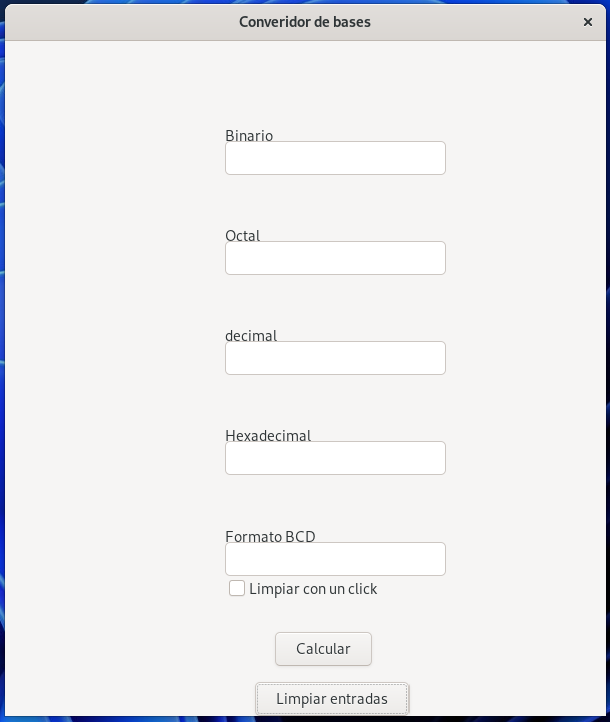
\includegraphics[width=7cm]{imag//ProgramDesign.png}
		\caption{Diseño del programa}
		% Convertidor
		\label{ProgramDesign}
		\end{center}
		%%\vspace{-1cm}
 		\end{figure}

		Para limpiar los campos de entrada de texto se crearon dos formas, una mediante
		un botón, y otra a través de un clic sobre cualquiera de los campos. El cambio de 
		método se da a través del check con la leyenda: Limpiar con un clic.
		
		Para el proceso de conversión se existen muchas formas de realizarlo, sin embargo
		se observó que pasar de Decimal a Binario, Octal y Hexadecimal se debe dividir el número
		decimal entre la base solicitada e ir concatenando los módulos de cada división
		hasta obtener cero, como se muestra en la figura \ref{decToOct}, donde se convierte de decimal
		a octal.

		% Coloca imagen de diseño de imagen
		\begin{figure}[H]
		\begin{center}
		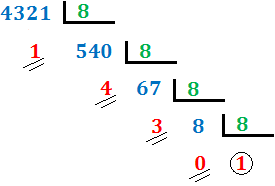
\includegraphics[width=7cm]{imag//decimalToOctal.png}
		\caption{Decimal a Octal}
		% Convertidor
		\label{decToOct}
		\end{center}
		%\vspace{-1cm}
		\end{figure}

		Con dicha forma de convertir las bases desde un número decimal se llegó a un algoritmo el cual
		convierte desde decimal a octal, binario y Hexadecimal, además de mostrar el resultado al usuario
		y de forma opcional regresarlo mediante un return en caso de ser necesario, el cual se muestra en la 
		figura \ref{algDecToRest}.

		% Coloca imagen de diseño de imagen
		\begin{figure}[H]
			\begin{center}
			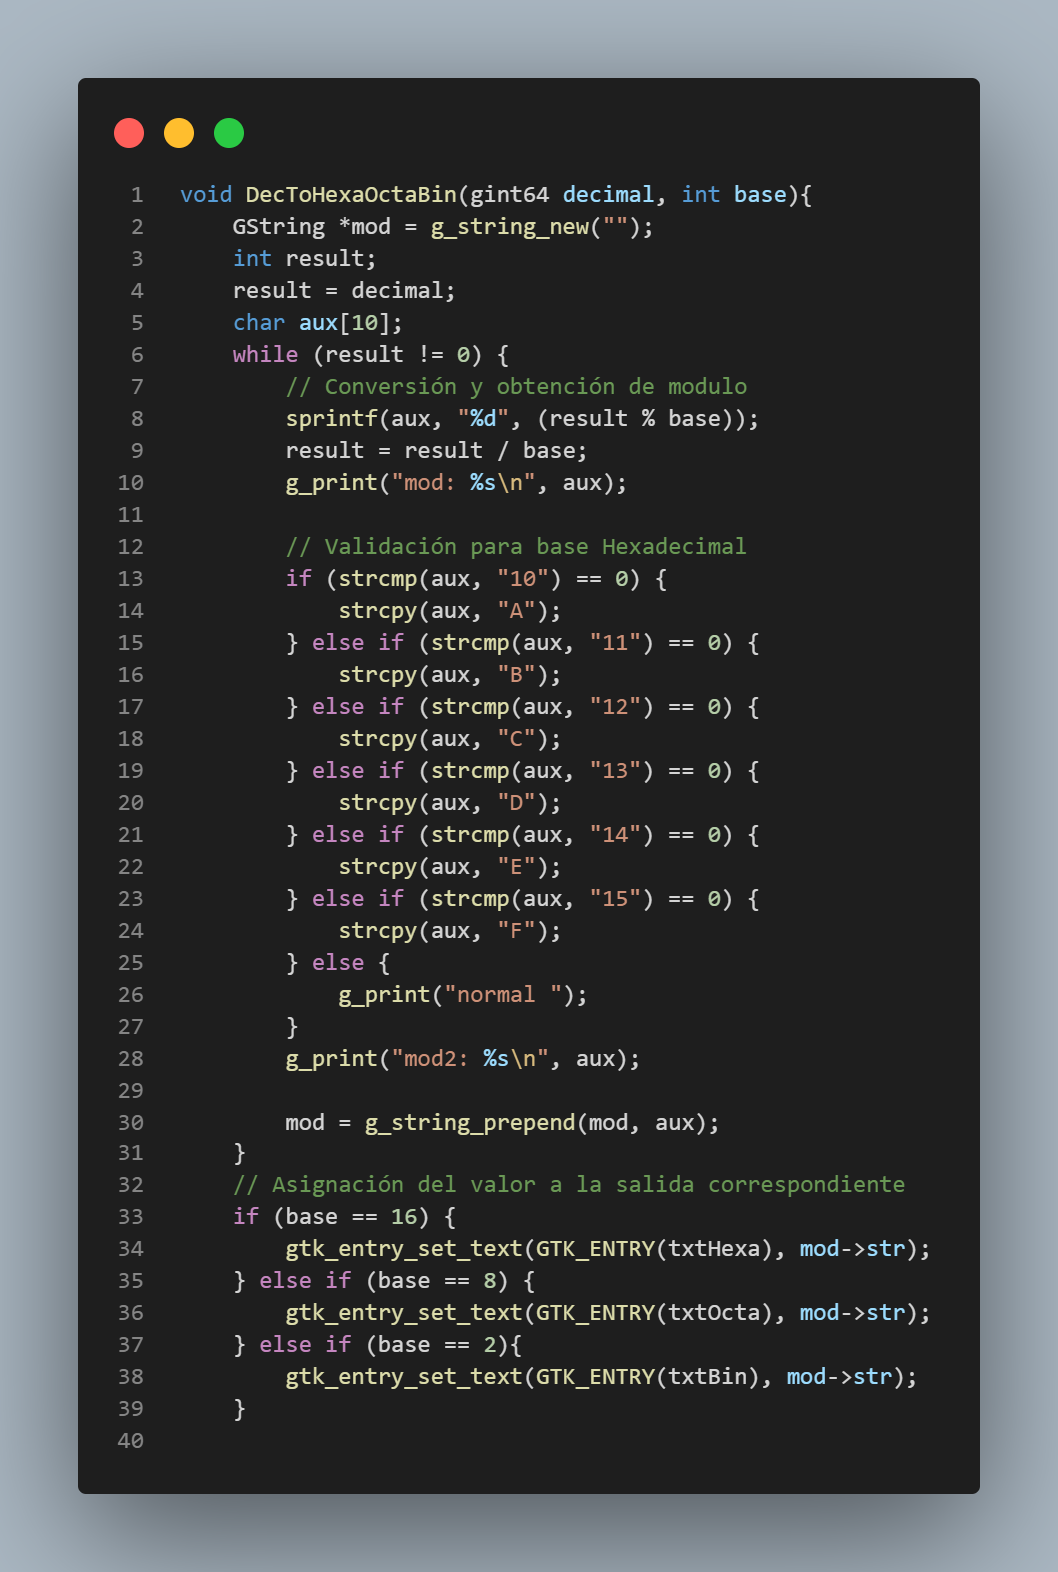
\includegraphics[width=10cm]{imag//algDecToRest.png}
			\caption{Algoritmo de conversión de bases}
			% Convertidor
			\label{algDecToRest}
			\end{center}
			%\vspace{-1cm}
			\end{figure}

			Con  el uso de este algoritmo solamente faltaría pasar de base Octal,
			Binario y Hexadecimal a binario, una vez echo esto el programa estaría
			casi completo, por lo que el primero en desarrollarse será de Binario a 
			Decimal. Lo primero que se realizó fue buscar el punto decimal en la 
			cadena binaria para futuras versiones. En este caso solo nos centraremos
			en los números enteros. Una vez que tenemos una cadena binaria entera
			se recorre de derecha a izquierda para ir elevando la base a su potencia 
			correspondiente. Figura \ref{algBinToDec} 
			
			% Coloca imagen de diseño de imagen
			\begin{figure}[H]
			\begin{center}
			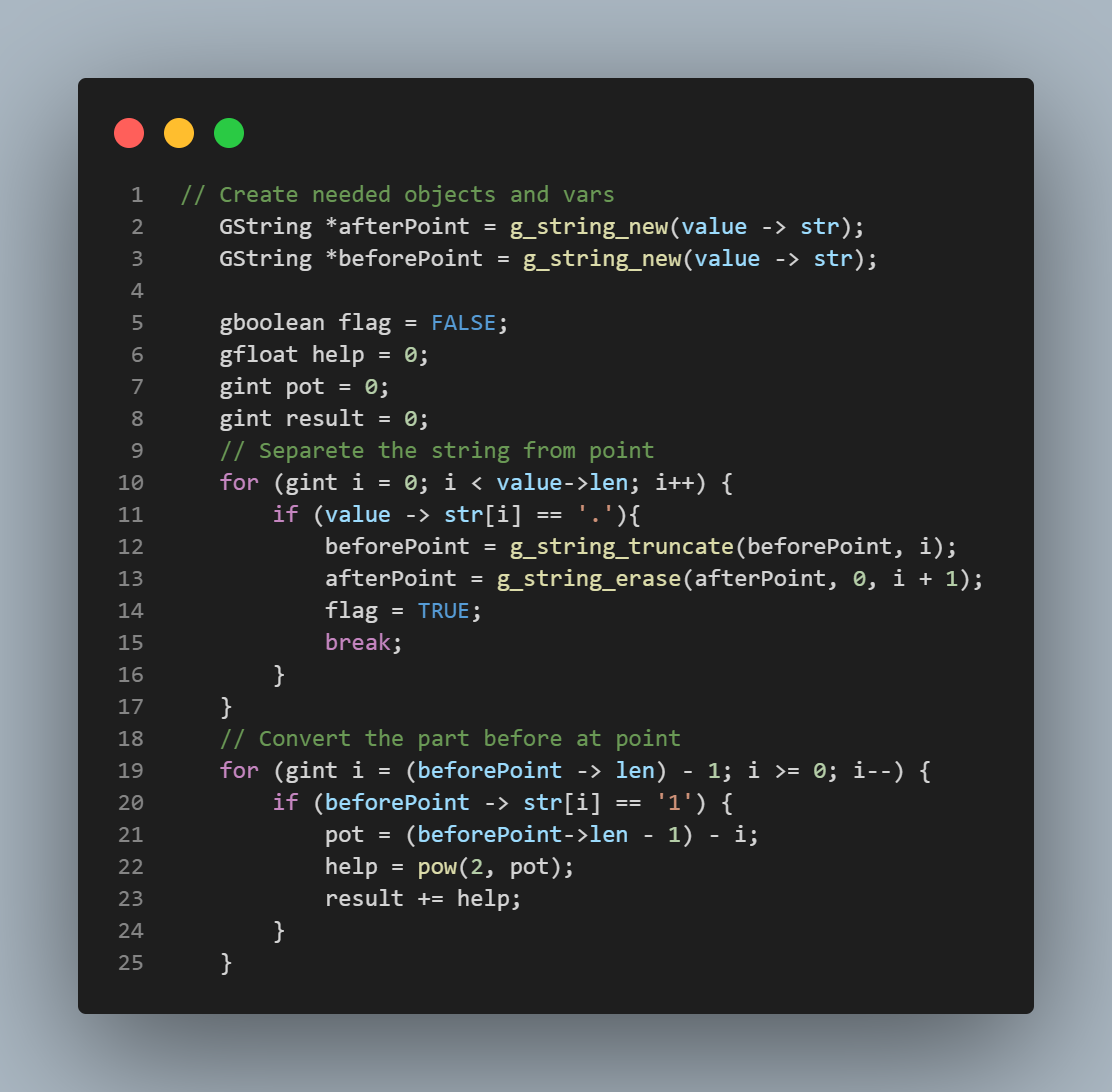
\includegraphics[width=9cm]{imag//algBinToDec.png}
			\caption{Algoritmo de binario a decimal}
			% Convertidor
			\label{algBinToDec}
			\end{center}
			%\vspace{-1cm}
			\end{figure}

			El resto de los algoritmos que convierten a binario se realizaron de forma similar. Una vez que fue
			posible convertir a decimal se utilizó el algoritmo de la figura \ref{algDecToRest} para llegar a las 
			demás bases.

			Para el formato BCD primero tenemos que tomar en cuenta que la cadena binaria se divide en grupos de 
			4 elementos para posteriormente transformarlos a decimal de forma separada y concatenar dichos números para 
			obtener el resultado.

			Se desarrolló un algoritmo que asegura que la cadena contendrá grupos de 4 elementos, posteriormente utiliza 
			el mismo algoritmo de conversión de Binario a Decimal (figura \ref{algBinToDec}) por grupos de 4 en 4 elementos.
			Por último concatena los resultados separados y muestra el resultado. Algoritmo en la figura \ref{algBcdToDec}.
			De forma adicional se transformó el formato bcd a Octal, Binario y Hexadecimal utilizando la función de la figura 
			\ref{algDecToRest} y el valor decimal obtenido.

			% Coloca alg de BCD a decimal
			\begin{figure}[H]
			\begin{center}
			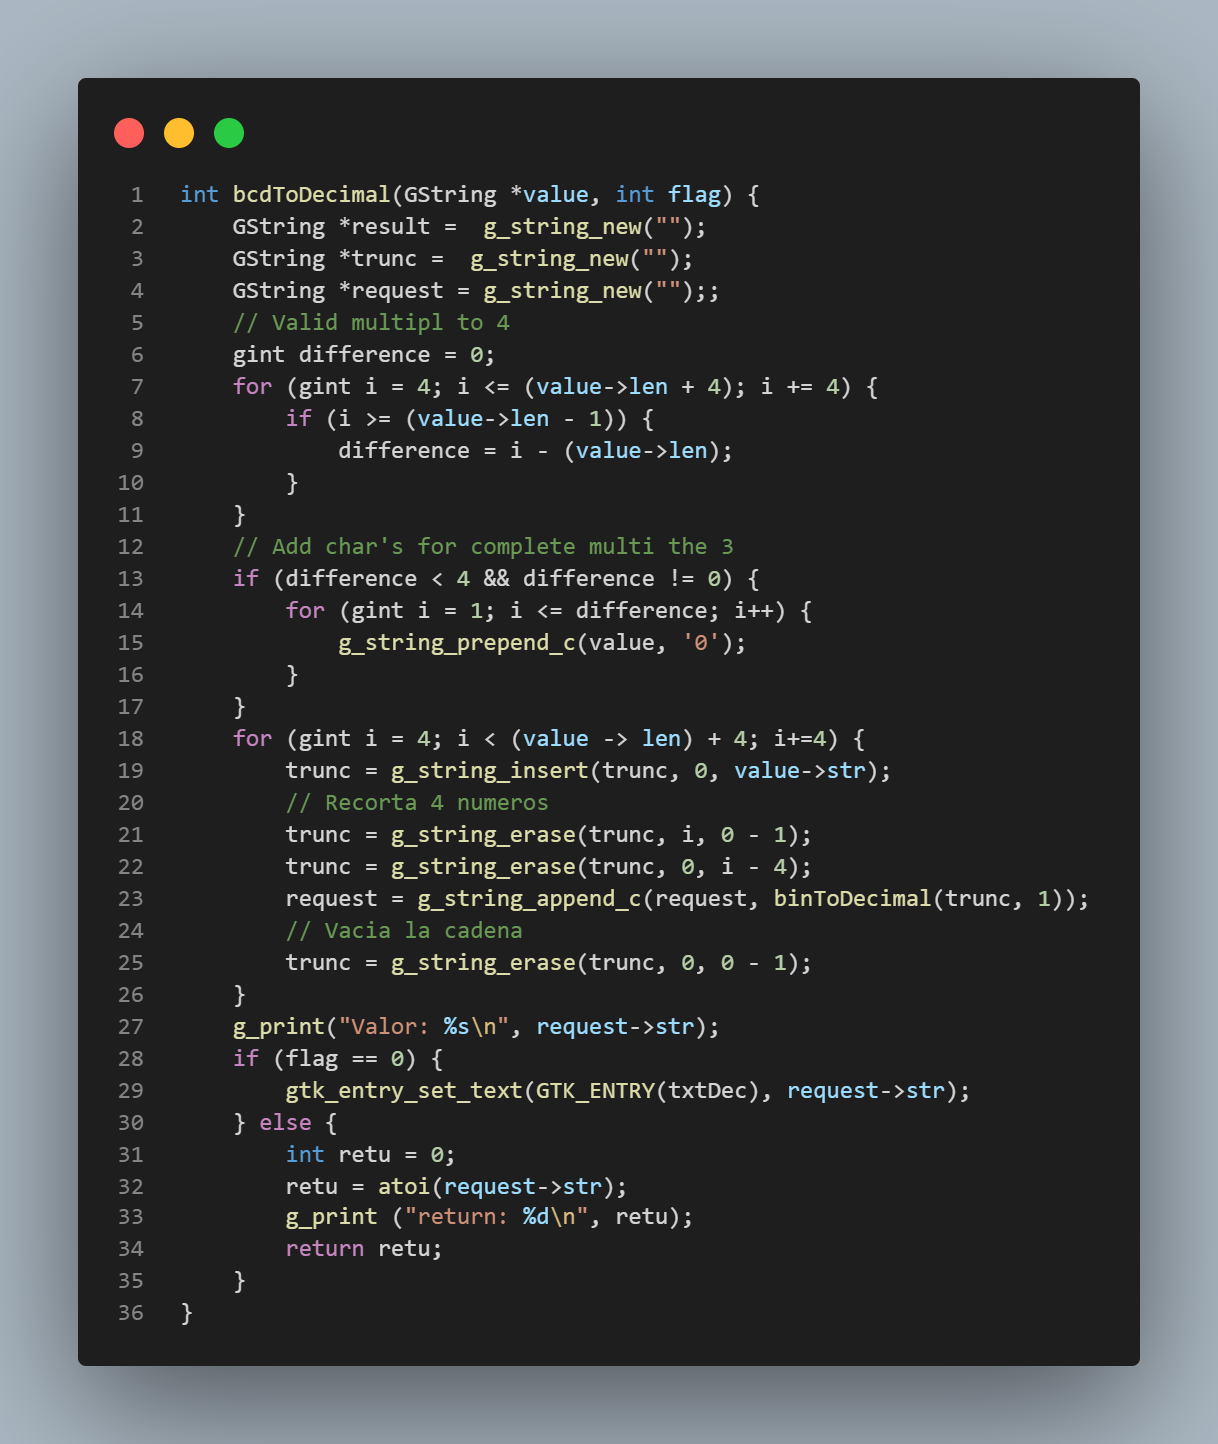
\includegraphics[width=10cm]{imag//algBcdToDec.png}
			\caption{Algoritmo de BCD a decimal}
			% Convertidor
			\label{algBcdToDec}
			\end{center}
			%\vspace{-1cm}
			\end{figure}

			Para convertir de los demás formatos a BCD se utiliza un algoritmo que los convierte a base decimal, donde  para 
			pasar de decimal a BCD se realizó un algoritmo que convierte decimal a formato BCD, como se muestra en la figura 
			\ref{decToBcd}. Es posible reutilizar dicho algoritmo para convertir de las demáss bases a formato BCD pasando por
			la base decimal y así obtener su equivalente. 

			% Coloca alg de BCD a decimal
			\begin{figure}[H]
			\begin{center}
			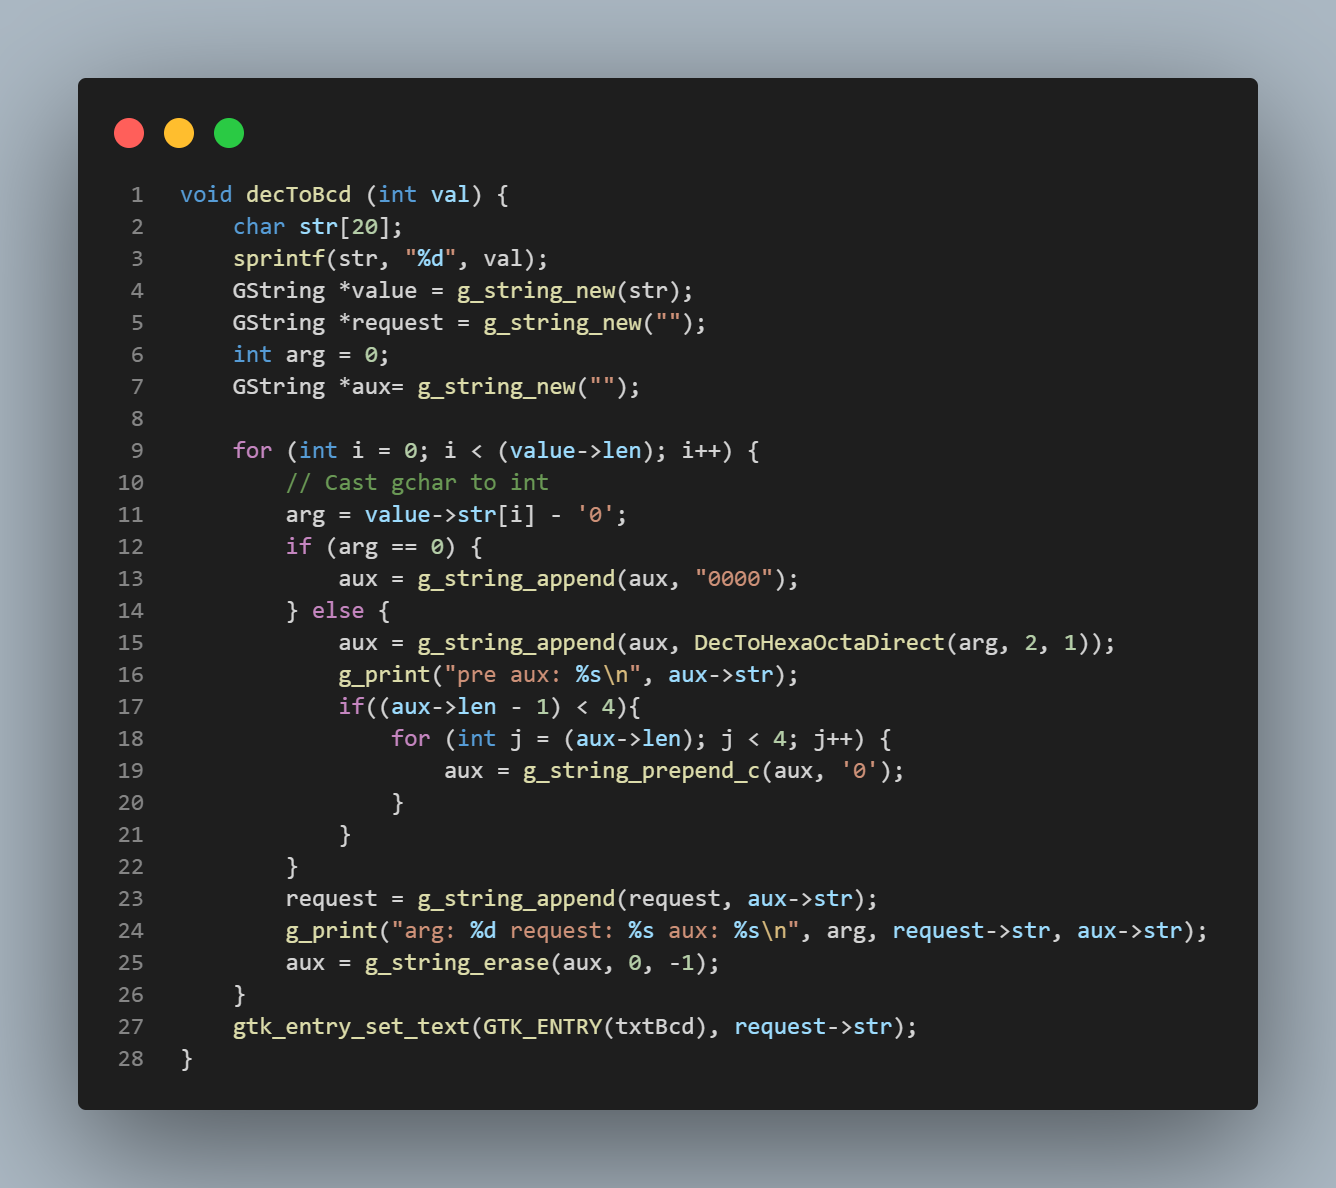
\includegraphics[width=9cm]{imag//algDecToBcd.png}
			\caption{Algoritmo de decimal a BCD}
			% Convertidor
			\label{decToBcd}
			\end{center}
			%\vspace{-1cm}
			\end{figure}
	
	\renewcommand{\labelenumi}{\arabic{enumi}.}
    
    	
    \section{Resultados}
		El programa actúa según lo esperado, siendo capaz de convertir de cualquier base al resto (dentro de las admitidas. Figura \ref{programFuntion}).
		Aún es posible mejorar el código utilizando otras herramientas que nos provee C, además de agregar aperaciones al programa
		como lo son la suma, resta, etc. Pero los objetivos para este proyecto se cumplieron. El código fuente se encuentra al final del archivo donde se
		estarán publicando las próximas versiones.		
		% Coloca alg de BCD a decimal
		\begin{figure}[H]
		\begin{center}
		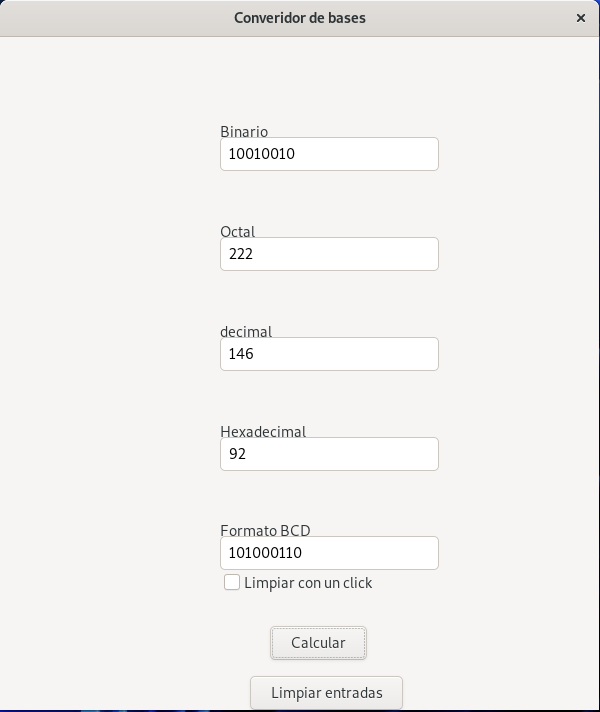
\includegraphics[width=9cm]{imag//programFuntion.png}
		\caption{Muestra de función del programa finalizado}
		% Convertidor
		\label{programFuntion}
		\end{center}
		%\vspace{-1cm}
		\end{figure}

	    \end{multicols}
	    \section{Conclusiones}
		El programa se completó con éxito, si bien no se realizaron conversiones entre algunas bases
		de forma directa, el objetivo del programa es poder realizar el cambio de base de un número de
		la manera más eficiente posible, que es lo que se realizó en dicho algoritmo, reciclar y generalizar
		un algoritmo para mejorar su legibilidad y eficiencia.
		
		Código fuente: \url{https://github.com/UnsisWorks/convert_base_gtk}
    
	\newpage
	
	% \section{Anexo de ecuaciones}
	
	% En caso des ser necesario se deben agregar ecuaciones que se hayan empleado

	% %Agrega todo lo ingresado tal cual
	% \begin{verbatim}
	% 	!"##$$%&%&/()
	% \end{verbatim}

	\cfoot{\LaTeX}
\end{document}